\documentclass[a4paper]{scrreprt}

\usepackage[utf8x]{inputenc}
\usepackage[OT1]{fontenc}
\usepackage[ngerman]{babel}
\selectlanguage{ngerman}
\usepackage{graphicx}
\usepackage{geometry}
\geometry{top=25mm,bottom=25mm,left=30mm,right=25mm}
\usepackage{setspace}
\onehalfspacing
\usepackage{color}

\usepackage{amsmath}
\usepackage{amssymb}

\usepackage[pdfpagelabels]{hyperref}
\hypersetup{colorlinks=false,pdfborder= 0 0 0}

\usepackage{booktabs}

\usepackage{xspace}
\renewcommand{\vec}[1]{\mathbf{\boldsymbol{#1}}}
\newcommand{\mat}[1]{\mathbf{#1}}
%\newcommand{\diag}{\mathrm{diag}}
%\newcommand{\trace}{\mathrm{trace}}
\newcommand\equationname{Eq.}
\newcommand\eg{\textit{e.g.},\xspace}
\newcommand\ie{\textit{i.e.},\xspace}
\newcommand\cf{\textit{cf.}\xspace}
\newcommand{\pderiv}[2]{\frac{\partial #1}{\partial #2}}
\newcommand{\pderivk}[3]{\frac{\partial^{#3} #1}{\partial #2^{#3}}}
\newcommand{\deriv}[2]{\frac{\operatorname{d} #1}{\operatorname{d} #2}}
\newcommand{\derivk}[3]{\frac{\operatorname{d}^{#3} #1}{\operatorname{d} #2^{#3}}}
\newcommand{\integral}[4]{\int_{#3}^{#4} #1 \operatorname{d}#2}
%\newcommand{\argmax}{\operatorname{argmax}}
%\newcommand{\argmin}{\operatorname{argmin}}
%\newcommand{\sign}{\operatorname{sign}}
\newcommand{\smalleq}{{\scriptstyle =}}
\newcommand{\quotes}[1]{``#1''}
\newcommand\landau{\mathcal{O}}
\newcommand\CONDON{\,|\,}
\newcommand{\vectornorm}[1]{\left|\left|#1\right|\right|}
\newcommand\kernelFunctionHIK{\kernelFunction^{\text{\scriptsize HIK}}}
\newcommand\kernelFunctionGHIK{\kernelFunction^{\text{\scriptsize GHIK}}}

\newcommand\mattwo[4]{\left[\begin{array}{cc} #1 & #2\\ #3 & #4 \end{array} \right]}
\newcommand\matthree[9]{\left[\begin{array}{ccc} #1 & #2 & #3\\ #4 & #5 & #6\\ #7 & #8 & #9 \end{array} \right]}
\newcommand\vectwo[2]{\left[\begin{array}{c} #1 \\ #2 \end{array} \right]}
\newcommand\vecthree[3]{\left[\begin{array}{c} #1 \\ #2 \\ #3 \end{array} \right]}

% notations

\DeclareMathOperator{\x}{\boldsymbol{x}}
\DeclareMathOperator{\y}{\boldsymbol{y}}

\newcommand\labelspace{\mathcal{Y}}
\newcommand\inputspace{\mathcal{X}}
\newcommand\inputsingle{\vec{x}}
\newcommand\inputsinglecomp{x}
\newcommand\labelsingle{y}
\newcommand\labelspecific{k}
\newcommand\labelrandom{\labelsingle}
\newcommand\inputrandom{\inputsingle}
\newcommand\dataset{\mathcal{D}}

\newcommand\dimension{D}
\newcommand\noe{n}
\newcommand\numberOfExamples{\noe}

\newcommand\inputnew{\inputsingle^*}
\newcommand\labelnew{\labelsingle_*}
\newcommand\inputmatrix{\mat{X}}
\newcommand\expectation{\mathbb{E}}
\newcommand\cfunction{\tilde{h}}
\newcommand\cestimate{\hat{h}}
\newcommand\impuls[1]{\delta\left[#1\right]}

\usepackage{upgreek}
\newcommand\impulsDiscrete[1]{\updelta \left( {#1} \right)}

\newcommand\numberOfClasses{M}
\newcommand\error{\mbox{\textit{err}}}


% model selection
\newcommand\cparameters{\vec{\theta}}
\newcommand\parameterspace{\Theta}

\newcommand\labelvector{\vec{y}}
\newcommand\inputdataset{\mat{X}}

% kernel stuff
\newcommand\meanFunction{\mu}
\newcommand\kernelFunction{K}
\newcommand\kernelMatrix{\mat{K}}
\newcommand\kernelMatrixValue{K}
\newcommand\kernelVector{\vec{k}_{*}}
%\newcommand\kernelVector{\kernelFunction(\inputdataset, \inputnew)}
\newcommand\kernelSelf{\kernelFunction(\inputnew, \inputnew)}

% latent functions
\newcommand\latentFunction{f}
\newcommand\latentvector{\vec{f}}
\newcommand\latentfunctionvalue{f}
\newcommand\latentnew{f_*}
\newcommand\ftransform{\phi}
\newcommand\distance{d}
\newcommand\rbfparameter{\gamma}
\newcommand\featureSpace{\mathcal{H}}
\newcommand\gpsymbol{\mathcal{GP}}
\newcommand\meanfunction{\mathcal{M}}

% model and modelspace / hypothesis, hypothesispace
\newcommand\hypothesis{h}
\newcommand\hypothesisSpace{\mathbb{H}}

\newcommand\mapestimate[1]{ {\hat{#1}}^{\text{MAP}} }
\newcommand\mlestimate[1]{ {\hat{#1}}^{\text{ML}} }
\newcommand\bayesestimate[1]{ {\hat{#1}}^{\text{Bayes}} }
\newcommand\mmseestimate[1]{ {\hat{#1}}^{\text{MMSE}} }
\newcommand\mss[1]{\mbox{\scriptsize #1}}
\newcommand\baggingFraction{r_{\mss{B}}}

\newcommand\assumeeq{\stackrel{*}{=}}
\newcommand\assumepropto{\stackrel{*}{\propto}}

\newcommand\ensembleSize{T}
\newcommand\ensembleIndex{t}

\newcommand\dtthreshold{\zeta}
\newcommand\thresholdSet{Q}
\newcommand\featureindex{r}
\newcommand\rFeatureSet{\mathcal{R}}

\newcommand\leafNode{\vartheta}
\newcommand\numberOfLeaves{m_\ell}
\newcommand\node{v}

\newcommand\splitCriterion{\Gamma}
\newcommand\impurityMeasure{\mathcal{J}}
\newcommand\entropy{\mathcal{E}}

\newcommand\impurityThreshold{\xi_\impurityMeasure}
\newcommand\minexamplesThreshold{\xi_{\mss{n}}}
\newcommand\maxdepthThreshold{\xi_{\mss{d}}}

\newcommand\hyperplane{\vec{w}}
%\newcommand\stepFunction[1]{\delta^s\left[ #1 \right]}
\newcommand\stepFunction[1]{\mbox{sign}\left(#1\right)}

\newcommand\numberOfKernels{R}
\newcommand\bias{b}
\newcommand\margin{\mbox{mg}}
\DeclareMathOperator\maximize{\mbox{maximize}}
\DeclareMathOperator\minimize{\mbox{minimize}}

\newcommand\hingeLoss{H}
\newcommand\lagrangeDual{g}

\newcommand\hyperparameters{\vec{\eta}}
\newcommand\hyperparameter{\eta}
\newcommand\kernelweight{\beta}
\newcommand\kernelweights{\vec{\beta}}
\newcommand\variance{\sigma^2}
\newcommand\stddev{\sigma}
\newcommand\eigmax{\lambda_{\text{max}}}
\newcommand\eigmin{\lambda_{\text{min}}}

% GP related stuff
\newcommand\gpregmean{\mu_*}
\newcommand\gpregvariance{\sigma^2_*}
\newcommand\gpregstddev{\sigma_*}

% differential symbol for integrals
\newcommand\diffd{d}

\newcommand\kernelscaling{v_0}
\newcommand\kernelbias{v_1}
\newcommand\qexpgrad{g}
%\newcommand\gpnoise{\sigma_{\varepsilon}^2}
\newcommand\gpnoise{\sigma^2}
\newcommand\gpnoisestddev{\sigma_{\varepsilon}}


%\newcommand\identityMatrix[1]{\mat{I}_{(#1)}}
\newcommand\identityMatrix[1]{\mat{I}}

\newcommand\kernelStuff{\zeta_\kernelFunction}

% gp classification
\newcommand\cumgauss{\Phi}
\newcommand\cumgaussLoss{L_{\cumgauss}}
\DeclareMathOperator\sigmoid{\mbox{sig}}
\newcommand\sigmoidLoss{L_{\scriptsize \text{sig}}}
\DeclareMathOperator\erf{\mbox{erf}}
% gp classification scaling factor
\newcommand\gpnoiseC{\sigma_{c}^2}
\newcommand\gpnoisestddevC{\sigma_{c}}

% laplace methods
\newcommand\laplaceMode{\vec{\hat{f}}}
\newcommand\laplaceModeValue{\hat{f}}
\newcommand\laplaceLog{L}
\newcommand\approxP{q}
\newcommand\constTerm{\text{\textit{const.}}}
\newcommand\nhessianLikelihood{\mat{W}}
\newcommand\nhessianLikelihoodValue{W}

% gp multi
\newcommand\ymulti{y_*^{\scriptsize \mbox{multi}}}
\newcommand\ymultip{y_*^{\scriptsize \mbox{multi}}}

% gp hyperparameter estimation
\newcommand\kernelMatrixHyper{\mat{\tilde{K}}_\hyperparameters}

% optimization problems

\newcommand\optimizationProblem[5]{
	\begin{equation}
	\label{#1}
	\begin{aligned}
	& \underset{#3}{#2}
	& & #4 \\
	& \text{subject to}
	& & #5 \enspace.
	\end{aligned}
	\end{equation}
}

\newcommand\optimizationProblemUnconstrained[4]{	
	\begin{equation}
	\label{#1}
	\begin{aligned}
	& \underset{#3}{#2}
	& & #4 \enspace.\\
	\end{aligned}
	\end{equation}
}
% transfer learning framework
%\newcommand\targetTask{\mathcal{T}}
\newcommand\targetTask{\tau}
\newcommand\supportTag{\mathcal{S}}
\newcommand\datasetSupport[1]{{\dataset}^{\supportTag}_{#1}}
\newcommand\datasetSupportSingle{{\dataset}^{\supportTask}}
\newcommand\datasetTarget{{\dataset}^{\targetTask}}
\newcommand\supportCollection{\mathfrak{D}^{\supportTag}}
\newcommand\numberOfTasks{J}
\newcommand\numberOfTasksMT{P}
\newcommand\noeTarget{\tilde{\noe}}
\newcommand\noeTotal{\noe}
\newcommand\noePositive{\noe_1}
\newcommand\noeSupport{\noe^{\supportTag}}
\newcommand\supportClasses{\supportTag}
\newcommand\supportClass{s}
\newcommand\backgroundClass{\mathcal{B}}
\newcommand\transferParameter{\vec{\theta}}
\newcommand\tpSpace{\Theta}

% regularized trees

\newcommand\targetClass{\targetTask}
\newcommand\rtPara{\vec{\theta}}
\newcommand\rtParaValue{\theta}
\newcommand\rtHyperMu{\vec{\mu}}
\newcommand\rtHyperMuValue{\mu}
%\newcommand\rtHyperSigma{\sigma_{\supportTag}}
\newcommand\rtHyperVariance{\sigma^2}
\newcommand\leafIndex{i}
\newcommand\datasetLeaf[1]{\omega_{#1}}
%\newcommand\datasetLeaf[1]{\dataset^{\ell}_{#1}}
%\newcommand\rtLeafProbs[1]{\vec{t}_{\supportTag}^{#1}}
\newcommand\rtLeafProbs[1]{\vec{t}^{(#1)}}
\newcommand\rtLeafProb[2]{t^{(#1)}_{#2}}
\newcommand\lagrange{L}
%\newcommand\mcdata[1]{\dataset^{#1}}
\newcommand\mcdata[1]{\dataset^{#1}}
%\newcommand\rtML[2]{\hat{\theta}^{\mss{(ML)},#2}_{#1}}
\newcommand\rtML[2]{t^{(#1)}_{#2}}
\newcommand\rtMLv[1]{\vec{t}^{(#1)}}
\newcommand\rtParaSpace{\Theta}

% only for the target task
\newcommand\rtMAPv{\vec{\hat{\theta}}^{\mss{MAP}}}

\newcommand\leafCounts{\vec{c}}
\newcommand\leafCount{c}
\newcommand\leafNodeBinaryV{\ftransform}
\newcommand\rtPostProbsV[1]{w^{\left(#1\right)}}
\newcommand\leafNodeBinary{\ftransform}
\newcommand\rtPostProbs[1]{\vec{w}^{\left(#1\right)}}

% feature relevance
\newcommand\featureSet{\mathcal{F}}
\newcommand\featureFunction{g}
\newcommand\frPara{\vec{\theta}}
\newcommand\frParaValue{\theta}
\newcommand\frBaseModel{h}
\newcommand\frBaseModelSpace{H}
\newcommand\frHyper{\vec{\beta}}
\newcommand\frHyperValue{\beta}
%\newcommand\

% depgp
\newcommand\depgpcorr{\rho}
\newcommand\tT{\textcolor{green}{\targetTask}}
\newcommand\tS{\textcolor{blue}{\supportTask}}
%\newcommand\supportTask{\supportTag}
\newcommand\supportTask{s}

\newcommand\depgpKNoColor{
	\left(\begin{array}{cc} \kernelMatrix_{\targetTask \targetTask} & \depgpcorr \kernelMatrix_{\targetTask \supportTask}\\ \depgpcorr \kernelMatrix_{\targetTask \supportTask}^T & \kernelMatrix_{\supportTask \supportTask}\end{array}\right)
}

\newcommand\depgpK{
		\LARGE\left(\begin{array}{cc} \kernelMatrix_{\tT \tT} & \depgpcorr \kernelMatrix_{\tT \tS}\\ \depgpcorr \kernelMatrix_{\tT \tS}^T & \kernelMatrix_{\tS \tS}\end{array}\right)
}
\newcommand\depgpKNoColorInd{
	\left(\begin{array}{cc} \kernelMatrix_{\targetTask \targetTask} & \mat{0}\\ \mat{0} & \kernelMatrix_{\supportTask \supportTask}\end{array}\right)
}

\newcommand\kernelFunctionX{\kernelFunction^{\inputspace}}
\newcommand\kernelMatrixX{\kernelMatrix^{\inputspace}}
\newcommand\kron{\otimes}
\newcommand\taskIndex{j}

\newcommand\kernelVectorTarget{\vec{k}_{\targetTask*}}
\newcommand\kernelVectorSupport{\vec{k}_{\supportTask*}}
\newcommand\labelvectorTarget{\labelvector_{\targetTask}}
\newcommand\labelvectorSupport{\labelvector_{\supportTask}}
\newcommand\inputdatasetTarget{\inputdataset_{\targetTask}}
\newcommand\inputdatasetSupport{\inputdataset_{\supportTask}}
\newcommand\loovariance{\tilde{\sigma}^2}
\newcommand\loomean{\tilde{\mu}}

\newcommand\kF{\mat{K}^{\latentfunction}}
\newcommand\kFTasks[2]{K^{\latentfunction}_{#1 #2}}
\newcommand\latentfunctionS{\tilde{\latentfunction}}
\newcommand\kernelFunctionS{\tilde{\kernelFunction}}
\newcommand\latentfunctionB{\bar{\latentfunction}}
\newcommand\kernelFunctionB{\bar{\kernelFunction}}
\newcommand\pilonettoWeight{\alpha}

\newcommand\wnsim{d}

% ------ tommasi
\newcommand\tommasiBeta{\beta}
\newcommand\hyperplaneTarget{\hyperplane^{(\targetTask)}}
\newcommand\hyperplaneSupport{\hyperplane^{(\supportTask)}}
\newcommand\alphaSupport{\vec{\alpha}^{(\supportTask)}}
\newcommand\alphaTarget{\vec{\alpha}^{(\targetTask)}}
\newcommand\alphaTargetValue{\alpha^{(\targetTask)}}

% ------ occ
\newcommand\occScore{\nu}
\newcommand\occThreshold{\xi}

\newcommand\ftMatrix{\mat{\Phi}}
\newcommand\kernelMatrixReg{\kernelMatrix_{\mss{reg}}}
\newcommand\covarianceReg{\mat{C}_{\mss{reg}}}
\newcommand\covarianceMatrix{\mat{C}}
\newcommand\ftmean{\vec{\mu}_{\ftMatrix}}
\newcommand\ftransformC{\tilde{\ftransform}}
\newcommand\squashFunction{\Phi}

\newcommand\radiusBall{R}
\newcommand\meanBall{\vec{m}}

% ------- local features

\newcommand\dimensionLF{S}
\newcommand\localfeature{\vec{l}}
\newcommand\lfposition{\vec{p}}
\newcommand\numberOfLFeat{W}
\newcommand\lfSet{\mathcal{L}}

% -------------- comparing histograms

\newcommand\setA{\mathcal{A}}
\newcommand\setB{\mathcal{B}}
\newcommand\baseSet{\mathcal{U}}
\newcommand\powerSet[1]{\mathcal{P}\left(#1\right)}
\newcommand\distSet{d}
\newcommand\clusterq{q}
\newcommand\numberOfClusters{n_q}

% -------------- BoF

\newcommand\bofHist{\vec{h}}
\newcommand\bofHistValue{h}
\newcommand\bofIndex{j}

% -------------- SIFT
\newcommand\aimg{\mathfrak{g}}
\newcommand\apoint{\vec{p}}
\newcommand\gaussianFilter[1]{\mathfrak{h}_{#1}}
\newcommand\gaussianScale{\sigma}
\newcommand\illuminationFunction{u}
\newcommand\greyValue{g}
\newcommand\conv{*}

% --------- pyramid matching
\newcommand\matchingError{\error_{\pi}}
\newcommand\pmkLevel{\ell}
\newcommand\numPMKLevels{L}
\newcommand\pmkHist{\vec{h}}
\newcommand\pmkHistValue{h}
\newcommand\pmkData{\mat{H}}
\newcommand\pmkSimilarity{\kernelFunction^{\mss{PMK}}}
\newcommand\pmkSimilarityNormalized{\tilde{\kernelFunction}^{\mss{PMK}}}
\newcommand\pmkMatches{I}

% --------- experiments
\newcommand\numRuns{Z}
\newcommand\confusionMatrix{\mat{C}}
\newcommand\confusionMatrixValue{C}
\newcommand\noeTest{\noe^{\mss{t}}}
%\newcommand\recogRate{\error^{\mss{ov}}}
%\newcommand\avgRecogRate{\error^{\mss{avg}}}
\newcommand\recogRate{\text{err-ov}}
\newcommand\avgRecogRate{\text{err-avg}}

\newcommand\ctp{\text{TP}}
\newcommand\cfp{\text{FP}}
\newcommand\cfn{\text{FN}}
\newcommand\ctn{\text{TN}}
\newcommand\numPositives{\noe_{\mss{pos}}}
\newcommand\numNegatives{\noe_{\mss{neg}}}
\newcommand\tprate{\text{TPR}}
\newcommand\fprate{\text{FPR}}


% define everything for a nice header
\usepackage{scrpage2}
\pagestyle{scrheadings}
% header also on first page of new chapter
\renewcommand*{\chapterpagestyle}{scrheadings} 
% font of header
\renewcommand{\headfont}{\normalfont}
% header
\ihead{
\includegraphics[width=0.1\linewidth]{img/hanfried-en-blue}}
 \chead{}
\ohead{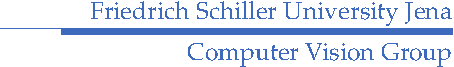
\includegraphics[width=0.3\linewidth]{img/fsuText-en}}
\setlength{\headheight}{21mm} % height of header

\title{Tutorial for GP-HIK-CORE}
\author{Alexander Freytag, Erik Rodner \\ \url{firstname.lastname@uni-jena.de}}
\setlength{\itemsep}{-0.5em}

\newcommand{\confSection}[1]{\textit{Section: } #1}
\newcommand{\variable}[1]{\textit{Variable: } #1}
\newcommand{\variableType}[1]{\textit{Type: } #1}
\newcommand{\default}[1]{\textit{Default: } #1}
\newcommand{\infos}[4]{
	\begin{itemize}
	  \setlength{\itemsep}{-0.5em}
	  \item \confSection{#1}
	  \item \variable{#2}
	  \item \variableType{#3}
	  \item \default{#4}
	\end{itemize}
     }

\definecolor{darkred}{rgb}{0.5,0,0}

\begin{document}

\maketitle

\setlength{\parindent}{0pt}
\renewcommand{\chaptername}{chapter}

\chapter{Preface}
\label{chap:Preface}
This document shall help to quickly use the modul gp-hik-core\footnote{\url{https://github.com/cvjena/gp-hik-core}} of our library NICE\footnote{\url{https://github.com/cvjena/nice-core}}.
It is structured as follows: 

\paragraph{Chapter~\ref{chap:SetUp}: How to set-up the library} We briefly explain things to be regarded while setting up our library.

\paragraph{Chapter~\ref{chap:ParamConfig}: Parameters and Configurations}
In \chaptername~\ref{chap:ParamConfig} we give an overview of the majority of built-in parameters, explain their influence briefly and present default settings.

\paragraph{Chapter~\ref{chap:DemoProgs}: Demo-Programs and how to use them}
In \chaptername~\ref{chap:DemoProgs} we introduce some demo programs we created to show how to switch between some parameter settings.


%--------------- setup --------------------
\chapter{Setting up the library}
\label{chap:SetUp}


\textbf{Step 1: Obtain our main library}\newline
\texttt{git clone https://github.com/cvjena/nice-core.git}
\vspace{2em}

\textbf{Step 2: configure everything}\newline
\texttt{cd nice-core/} \newline
\texttt{source setenv.sh}
\vspace{2em}

\textbf{Step 3: Obtain the gp-hik-core module}\newline
\texttt{git clone https://github.com/cvjena/gp-hik-core.git}
\vspace{2em}

\textbf{Step 4: Build everything}\newline
\texttt{cd cd gp-hik-core/} \newline
\texttt{make}
\vspace{2em}

\textbf{Step 5: Verify that everything works properly}\newline
\texttt{make check}



%--------------- parameter configs -------------------- 
\chapter{Parameter Configurations}
\label{chap:ParamConfig}

\section{Classification in general}
  \paragraph{Specify the interative linear solver}
    \infos{GPHIKClassifier}{ils\_method}{string}{CG}
    \begin{tabular}{ll}
      \textbf{Setting} & \textbf{Explanation} \\
	CG     &  the conjugate gradients method\\
	CGL    &  the conjugate gradients method using Lanczos process \\
	SYMMLQ &  the symmetric LQ (SYMMLQ) method using Lanczos process\\
	MINRES &  the minimum residual method using Lanczos process \\
    \end{tabular}

  \paragraph{Specify the optimization method}
    \infos{GPHIKClassifier}{optimization\_method}{string}{greedy}
    \begin{tabular}{ll}
      \textbf{Setting} & \textbf{Explanation} \\
	greedy            &  greedy 1D search in a pre-defined range\\
	downhillsimplex   &  DHS in multiple dimensions \\
	none              &  no optimization at all\\
    \end{tabular}

\section{Classification with Quantization}
  \paragraph{(De-)Activate the Quantization}
    \infos{GPHIKClassifier}{use\_quantization}{bool}{false}
  \paragraph{Specify precision of quantization}
    \infos{GPHIKClassifier}{num\_bins}{integer}{$100$}

\section{Uncertainty Prediction}
\paragraph{Activate or de-active the computation of predictive uncertainties}
  \infos{GPHIKClassifier}{uncertaintyPredictionForClassification}{bool}{false}

\paragraph{Specify how to compute predictive uncertainties}
  \infos{GPHIKClassifier}{varianceApproximation}{string}{approximate\_fine}

  \begin{tabular}{ll}
    \textbf{Setting} & \textbf{Explanation} \\
      approximate\_rough &  use the RAPU method (perhaps with quantization, see our ACCV'12 paper)\\
      approximate\_fine &  use the FAPU method \\
      exact &  use the PUP method\\
      none &  deactivate the computation \\
  \end{tabular}


\section{Various}
% 
  \paragraph{Generalizations of HIK}
    \infos{GPHIKClassifier}{transform}{string}{absexp}

    \begin{tabular}{ll}
      \textbf{Setting} & \textbf{Explanation} \\
	absexp &  absolute value and exponential operation -- pow(fabs(x), exponent)\\
	exp &  exponential operation -- exp(fabs(x), exponent)\\
	MKL &  weights for Multiple Kernel Learning approach\\
	WeightedDim &  weights for each dimension\\
    \end{tabular}

  \paragraph{Useful Output}
    \infos{GPHIKClassifier}{verbose}{bool}{false}

  \paragraph{Computation Time Output}
    \infos{GPHIKClassifier}{verboseTime}{bool}{false}

  \paragraph{Useful Debug Output}
    \infos{GPHIKClassifier}{debug}{bool}{false}

\section{GP related settings}
  \paragraph{Set the GP noise for model regularization}
    \infos{GPHIKClassifier}{noise}{double}{$0.01$}
  \paragraph{(De-)Activate balanced learning}
    \infos{GPHIKClassifier}{learn\_balanced}{bool}{false}
  \paragraph{(De-)Activate aumatic determination of noise}
    \infos{GPHIKClassifier}{optimize\_noise}{bool}{false}


% \chapter{Class Structure}


\chapter{Demo Programs}
\label{chap:DemoProgs}

\section{Toy Example for Classification}

A simple toy example with synthetic data can be run with the program  \texttt{toyExample}. You may call the program with a default configuration via 

  \texttt{../BUILD\_x86\_64/gp-hik-core/progs/toyExample -config ./configs/toyExample.conf}.

\paragraph{Usage and Accuracies}
This program uses synthetic data of $3$ classes with $49$ dimensions. For training, $20$ examples per class are used, whereas we provide $50$ examples per class for testing. 

Without any changes, you should obtain an accuracy of $99.33\%$. If you activate the quantization approach (either in the config file or via 
\texttt{-GPHIKClassifier:use\_quantization true}) the accuracy drops to $89.33\%$ since the sampled features cover small ranges in the input space. However, 
when increasing the number of quantization steps to $1,000$, the resulting accuracy is again $99.33\%$.

\paragraph{Quantization: Runtimes and Memory}
When switching between with and without quantization, you should notice the differences in resulting runtimes. On our computer (single core, $3.4$GHz), 
we obtain the following results:

\begin{center}
 \begin{tabular}{ccccc}
    \textbf{Quantization} & \textbf{Training [s]} & \textbf{Testing [s]} & \textbf{Memory [kB]} & \textbf{Accuracy [\%]}\\
     \hline
    no                    & $5.06$                & $0.19$               & $26,228$             &  $99.33$\\
    yes, $100$            & $5.09$                & $0.01$               & $26,488$             &  $89.33$ \\
    yes, $1,000$          & $5.13$                & $0.01$               & $27,540$             &  $99.33$ \\
  \end{tabular}
\end{center}

\section{Evaluation of Fast Min Kernel}
\begin{itemize}
 \item Name of Program
    \begin{itemize}
      \item[ ] \texttt{completeEvaluationFastMinkernel}
    \end{itemize}
 \item Input:
    \begin{itemize}
      \item[\texttt{-n}] number of examples
      \item[\texttt{-d}] number of dimensions
      \item[\texttt{-v}] additional output
    \end{itemize}
 \item Usage: three main parts
    \begin{enumerate}
      \item initialization (FMK vs. computation of $\kernelMatrix$)
      \item kernel multiplication $\kernelMatrix \cdot \alpha $
      \item kernel sum $\kernelVector^T \cdot \alpha $
    \end{enumerate}
\end{itemize}

\chapter{Closing words}
This library was built to provide a fast and memory efficient possibility for bayesian inference in large-scale scenarios. 
The algorithms are published in the following papers.
\vspace{1em}

Large-scale classification (training, optimization, testing):
\begin{itemize}
  \item \textbf{Large-Scale Gaussian Process Classification with Flexible Adaptive Histogram Kernels} by \textit{Erik Rodner and Alexander Freytag and Paul Bodesheim and Joachim Denzler} (ECCV 2012. 85--98) and
\end{itemize}
Rapid uncertainty computation, incremental and active learning:
\begin{itemize}
  \item \textbf{Rapid Uncertainty Computation with Gaussian Processes and Histogram Intersection Kernels} by \textit{Alexander Freytag and Erik Rodner and Paul Bodesheim and Joachim Denzler} (ACCV 2012. ), which was awarded with the \textcolor{darkred}{\bf ``Best paper honorable mention''}.
\end{itemize}


In case of any problems or suggestions for improvement, don't hesitate to contact us.

\vspace{10em}
\begin{center}
  
\includegraphics[width=0.5\linewidth]{img/logoV2blue}
\end{center}


\end{document}